%%%%%%%%%%%%%%%%%%%%%%%%%%%%%%%%%%%%%%%%%%%%%%%%%%%%%%%%%%%%%%%%%%%%%%%%%%%%%%%
% Chapter 2: Título del capítulo 2
%%%%%%%%%%%%%%%%%%%%%%%%%%%%%%%%%%%%%%%%%%%%%%%%%%%%%%%%%%%%%%%%%%%%%%%%%%%%%%%

%++++++++++++++++++++++++++++++++++++++++++++++++++++++++++++++++++++++++++++++

%++++++++++++++++++++++++++++++++++++++++++++++++++++++++++++++++++++++++++++++
\section{Optimización Global}
\label{sec:OPT}
%%%%%%%%%%%%%%%%%%%%%%%%%%%%%%%%%%%%%%%%%%%%%%%%%%%%%%%%%%%%%%%%%%%%%%%%%%%%%%


La Optimización Global trata de optimizar una función dentro de un intervalo especificado y teniendo en cuenta diversos criterios y/o restricciones, como puede ser el caso de optimización multiobjetivo. Por lo general, el objetivo de la optimización global es la de encontrar el óptimo (mínimo o máximo) u óptimos globales de la función $f$ a optimizar, tratando de evitar posibles óptimos locales. 
La optimización global se basa en encontrar aquel valor mínimo o máximo global dentro del espacio de búsqueda de la función \textbf{\textit{f}} a optimizar. La elección de la técnica empleada para encontrar el óptimo global resulta de gran importancia dado que la función \textbf{\textit{f}} puede tener varios óptimos locales que pueden llevar al algoritmo a \textbf{converger prematuramente}, sin que luego pueda escapar de los mismos. \\
De manera formal, el objetivo de la optimización global, considerando un problema de minimización, es encontrar un vector $X* \in \Omega$ tal que $f(X*) \leq f(X)$ para todo $X \in \Omega$ \cite{Segredo2017}.
En este caso particular, tratamos la optimización de tipo \textbf{\textit{box-constrained}}, donde \textbf{el espacio de búsqueda} $\Omega$ está definido por un límite inferior ($a_{i}$) y superior ($b_{i}$) para cada una de las variables de decisión de la función, es decir: $\Omega = \prod^{D}_{i=1}[a_{i}, b{i}]$, siendo D el número de variables de decisión del problema a optimizar \cite{Segredo2017}.


%%%%%%%%%%%%%%%%%%%%%%%%%%%%%%%%%%%%%%%%%%%%%%%%%%%%%%%%%%%%%%%%%%%%%%%%%%%%%%
\section{Técnicas Meta-heurísticas}
\label{sec:META}
%%%%%%%%%%%%%%%%%%%%%%%%%%%%%%%%%%%%%%%%%%%%%%%%%%%%%%%%%%%%%%%%%%%%%%%%%%%%%%

Las meta-heurísticas son un sub-conjunto de métodos de optimización que se encuentran incluidas dentro del conjunto de métodos heurísticos que a su vez forman parte de los métodos aproximados.

\begin{figure}
  \centering
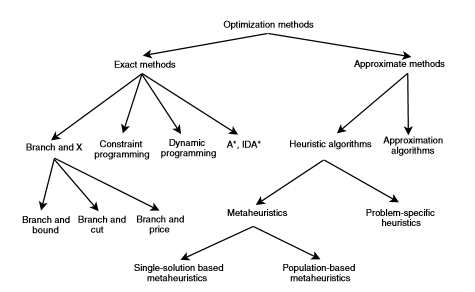
\includegraphics[scale=1.0]{images/meta}\\[10mm]
  \caption{Métodos de optimización.}
\end{figure}

A diferencia de los métodos de optimización exactos, las meta-heurísticas nos permiten obtener soluciones factibles a problemas complejos en un tiempo aceptable, aunque no nos garantizan obtener la solución óptima global \cite{metaheuristics}. En los últimos años estás técnicas algorítmicas han ganado una gran popularidad dado que han demostrado su efectividad y eficiencia en muchos campos y con una gran cantidad de problemas distintos.

En cuanto a las distintas meta-heurísticas que podemos encontrar hoy en día, podemos diferenciar las siguientes categorías \cite{metaheuristics}:

\begin{itemize}
    \item \textbf{Búsquedas Locales}: Greedy Randomized Adaptive Search Procedure (GRASP) \cite{GRASP}, Variable Neighborhood Search (VNS) \cite{vns}.
    \item \textbf{Heurísticas Voraces}: Simulated Annealing (SA) \cite{SA}.
    \item \textbf{Algoritmos Evolutivos}: Covariance Matrix Adaptation Evolutionary Strategy (CMA-ES) \cite{CMA}, Differential Evolution (DE) \cite{DE1, DE2, DE3}, Coevolutionary Algorithms (CEA) \cite{COE1, COE2, COE3}.
\end{itemize}


Esta gran variedad de técnicas se debe principalmente al gran abanico de criterios que podemos definir a la hora de diseñar una meta-heurística. Generalmente, las meta-heurísticas, y en especial, los algoritmos evolutivos, buscan un balance entre las propiedades de intensificación y diversificación. El concepto de intensificación significa aprovechar una solución prometedora  obtenida y tratar de explotar la región del espacio de búsqueda cercana a la misma en busca de posibles mejores soluciones, mientras que la diversificación se caracteriza por priorizar la búsqueda por las diferentes áreas no exploradas del espacio de búsqueda. Sin embargo, algunas técnicas como la búsqueda local, se centran principalmente en intensificar. Otra clasificación agrupa las diferentes meta-heurísticas en las siguientes clases \cite{metabook}:

\begin{itemize}
    \item \textbf{Métodos inspirados en la naturaleza}: es común inspirarse en el comportamiento de animales o bien de procesos físicos para diseñar un método meta-heurístico que emule ese comportamiento. Por ejemplo: Ant Bee Colonies \cite{Mann2017} y Simulated Annealing \cite{SA}.
    \item \textbf{Determinísticos o Estocásticos}: podemos optar por tomar decisiones deterministas o emplear reglas aleatorias durante la búsqueda de nuevas soluciones.
    \item \textbf{Métodos basados en poblaciones o basados en una única solución}: por un lado nos podemos basar en un conjunto de soluciones factibles que combinaremos entre ellas aplicando diversos operadores para obtener un  nuevo conjunto de soluciones potencialmente mejores. O bien, podemos optar por utilizar una única solución al problema que transformaremos en cada iteración del algoritmo.
    \item \textbf{Iterativos o voraces}: en este aspecto podemos contemplar comenzar con un conjunto de soluciones factibles al problema y transformar dichas soluciones en cada iteración del algoritmo para obtener nuevas soluciones con mejor evaluación. Al contrario, en una estrategia voraz (Greedy) comenzamos sin una solución factible al problema y en cada iteración incluiremos una variable de decisión hasta obtener una solución completa al problema \cite{metabook}. 
\end{itemize}

\subsection{Representación}

En las técnicas algorítmicas en general nos podemos encontrar con diversas maneras de representar la solución $S$ al problema y en las meta-heuristicas las siguientes son las más comunes \cite{metaheuristics}:

\bigskip

\begin{itemize}
    \item \textbf{Cadena binaria}: utilizada en problemas de decisiones.
    \begin{figure}[!ht]
    \centering
    
\includegraphics[scale=1.2]{images/binaria}
    \caption{Ejemplo de representación en cadena binaria.}
    \end{figure} 
    \item \textbf{Vector de valores naturales}: utilizada en problemas de optimización combinatoria.
    \begin{figure}[!ht]
    \centering
    
\includegraphics[scale=1.2]{images/natural}
    \caption{Ejemplo de representación en vector de números naturales.}
    \end{figure}
    \item \textbf{Vector de números reales}: utilizada en problemas de optimización continua.
    \begin{figure}[!ht]
    \centering
    
\includegraphics[scale=1.2]{images/reales}
    \caption{Ejemplo de representación en vector de números reales.}
    \end{figure}
    \item \textbf{Permutaciones}: empleada, por ejemplo en problemas de rutas y de planificación de tareas.
    \begin{figure}[!ht]
    \centering
    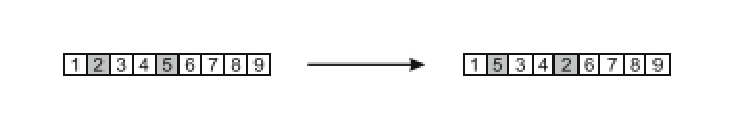
\includegraphics[scale=1.2]{images/secuencia}
    \caption{Ejemplo de representación en permutaciones.}
    \end{figure}
\end{itemize}

Dadas las características del concurso seleccionado para este Trabajo de Fin de Grado, la representación empleada fue \textbf{vector de valores reales} dado que cada elemento del vector denota un valor dentro del dominio de la función para cada una de las \textbf{\textit{D variables}} que posee.

\subsection{Condición de Parada}
Generalmente, las técnicas meta-heurísticas finalizan su ejecución según un criterio de finalización o \textbf{condición de parada}. Las más comunes son: 

\bigskip

\begin{itemize}
    \item \textbf{Iteraciones}: el algoritmo se detiene al alcanzar un determinado número de iteraciones.
    \item \textbf{Evaluaciones}: cuando el número de evaluaciones de la función objetivo a optimizar realizadas por el algoritmo llega a un valor prefijado, el algoritmo finaliza su ejecución.
    \item \textbf{Factor de error}: al alcanzar un factor de error lo suficientemente bajo como para considerar la solución óptima, el algoritmo detiene su ejecución.
\end{itemize}

En nuestro trabajo, el criterio de parada utilizado por todos los algoritmos desarrollados es \textbf{$10^{6}$ evaluaciones}, criterio prefijado por la organización del concurso GenOpt. 
